\documentclass{article}


\usepackage{arxiv}

\usepackage[utf8]{inputenc} % allow utf-8 input
\usepackage[T1]{fontenc}    % use 8-bit T1 fonts
\usepackage{hyperref}       % hyperlinks
\usepackage{url}            % simple URL typesetting
\usepackage{booktabs}       % professional-quality tables
\usepackage{amsfonts}       % blackboard math symbols
\usepackage{nicefrac}       % compact symbols for 1/2, etc.
\usepackage{microtype}      % microtypography
\usepackage{lipsum}
\usepackage{graphicx}
\graphicspath{ {./graphics/} }

\title{Video Games Ontology}


\author{
  Alexandre Dazat \\
  \texttt{alexandre.dazat@telecom-sudparis.eu} \\
  %% examples of more authors
   \And
  Julien Denize\\
  \texttt{julien.denize@telecom-sudparis.eu} \\
}

\begin{document}
\maketitle



% keywords can be removed

\section*{A Basics}

\subsection*{A.1 Ontology name}
Video-games ontology, v1.0 

\subsection*{A.2 Ontology owner}

Julien DENIZE, Alexandre DAZAT

\subsection*{A.3 Ontology license}

Creative Commons Attribution 3.0 (CC BY 3.0) 

\subsection*{A.4 Ontology URL}

https://github.com/juliendenize/Video-Games-Ontology/blob/master/ontology.owl


\subsection*{A.5 Ontology repository }

https://github.com/juliendenize/Video-Games-Ontology

\subsection*{A.6 Methodological framework}

No specific methodological framework has been used. Properties and classes selection were made to fit the context and requirements. 


\section*{B. Motivation}


\subsubsection*{B.1 Need}

Single ontology resource that enables users to look up for video games in databases with fine-grained granularity regarding the platforms, people involved in development, famous players and genres.

\subsection*{B.2 Competition}

The closest ontology to what we did can be found at the following URL : 
 
 
https://bartoc.org/en/node/18344

Besides, it mainly aims at encapsulating knowledge on events that happen in video games and information about players, whereas ours is made in order to store general information, as well as in depth features including genre or production team of games in order to retrieve it from large market databases.

\subsection*{B.3 Target audience}

The Video Game Ontology aim to be used by video game digital distribution service platforms such as Steam or Amazon to provide quality modeling in games representation so that consumers can provide the most accurate queries and get to the product they are looking for or discover interesting ones based on the various functional attributes available. 

\section*{C. Scope, requirements, development community}
\subsection*{C.1 Scope and coverage}
The ontology focuses on representing relevant features for consumers and users to be able to retrieve video games they are looking for. This goal requires to provide at least some key features : Genre, platform, PEGI. 

Indeed, one might also be searching for some games produced by their favourite video games company, or more specifically some well-known developer or sound designer. 

Besides, it is also likely that the rise of streaming platforms and e-sport paves the way for new consuming habits of people looking for games based on which games their favourite professional players or streamers broadcasts.

In this context, we extended the scope of the ontology by adding the following classes : Company, Job, Human (subclasses  in section [...])

The overall scope has been chosen in order to answer the type of questions one can find in section G.1 - Testing



\subsection*{C.2 Development community}
Alexandre DAZAT and Julien DENIZE
\subsection*{C.3 Communication}

https://github.com/juliendenize/Video-Games-Ontology
\section*{D. Knowledge acquisition}

\subsection*{D.1 Knowledge acquisition methodology}

Personal general knowledge acquired through 15+ years of gaming and structured into an ontology through the coursework given in IA301. 
\subsection*{D.2 Source knowledge location}
We collected data from Wikipedia and existing video games recommendation platforms (Steam, Amazon etc ..) 
\subsection*{D.3 Content selection}


In order to provide good quality representation the Video Games Ontology has to gather enough well-known games, production team leaders and games of diverse genre. The goal is to provide at least the means for retrieving the most commonly searched games, the more the database grows in individuals and the more consumers will find what they are looking for. 
\section*{E. Ontology content}

\subsection*{E.1 Knowledge Representation language}
OWL version 2, EL profile.  
\subsection*{E.2 Development environment}
Protégé 5.5.0
\subsection*{E.3 Ontology metrics}
\begin{figure}[h]
 \centering
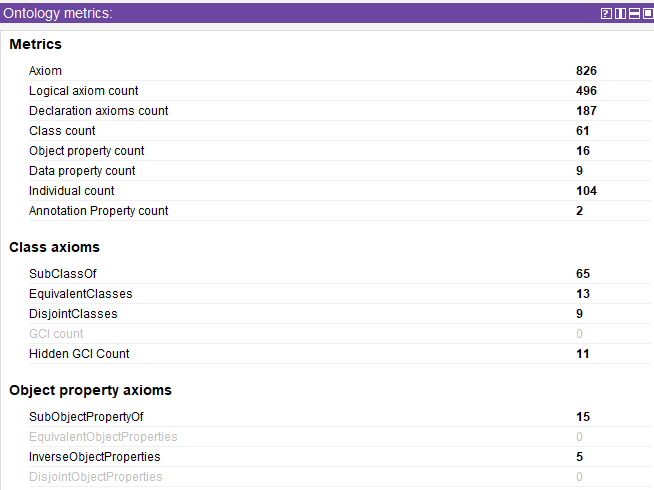
\includegraphics[scale=0.4]{Metrics1} 
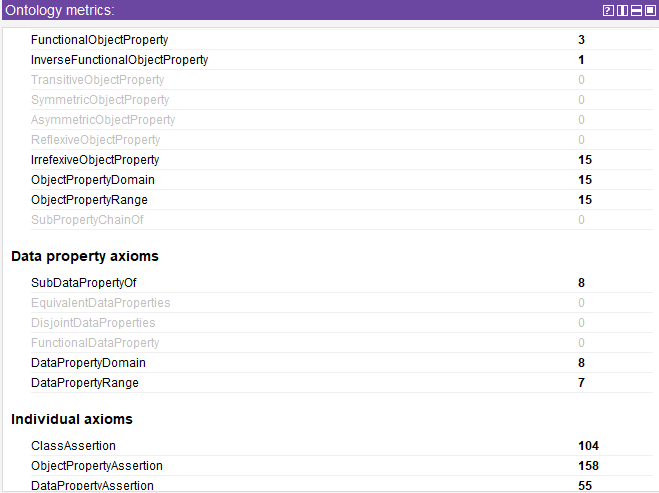
\includegraphics[scale=0.4]{Metrics2}
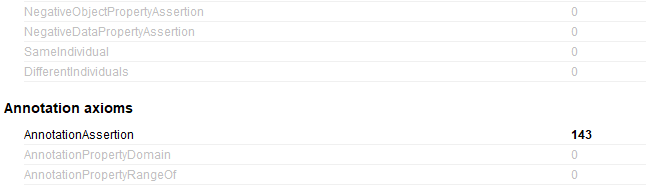
\includegraphics[scale=0.4]{Metrics3}
\end{figure}
\subsection*{E.4 Incorporation of other ontology's}
The ontology was made from scratch with no other ontology incorporated. 

\subsection*{E.6 Identifier generation policy}

Spaces are replaced by underscores in individual names. Properties and classes are named according to CamelCase norm. 
\subsection*{E.7 Entity metadata policy}
Each class and property has a description. 
\subsection*{E.8 Upper ontology}

No upper ontology has been used, the ontology was made from scratch
\subsection*{E.9 Ontology relationships}

We could have reused the Organization and product relationships from Schemas.org but the scope of the ontology made it hard to derive and adapt almost all properties for the use case. Instead we built our own model to fit the video games area. 

\begin{table}[h!]
\centering
 \begin{tabular}{| c c |} 
 \hline
Object property & Description \\ [0.5ex] 
 \hline\hline
 isEmployedBy & An employee is employed by a company  \\
 hasPlayed &  A player played a video game \\
 hasDeveloped & An employ develops video games \\
 hasEmployed & A company employ employees\\
 hasFounded & A company has been founded by an employee \\
 hasGender & A person has a gender   \\
 hasGenre & A video game can have multiple genres \\
 hasJob & An employee has one or several jobs   \\
 hasPEGI & A video game has a PEGI  \\
 hasPlatform & A video game has a platform \\
 hasProduced & A company has produced a video game\\
 isDevelopedBy & A video game is developed by an Employee \\
 isFoundedBy & A company is founded by an employee (inverse of hasFounded)  \\
 isPlayedBy & A video game is played by players (inverse of hasPlayed)  \\
 isProducedBy & A video game is produced by a company (inverse of hasProduced)  \\[1ex] 
 \hline
 \end{tabular}
\end{table}


\begin{table}[h!]
\centering
 \begin{tabular}{| c c c c c c c c c c |} 
 \hline
 Object Property & Func & InvFunc & Trans & Asym & Refl & Irrefl & Domain & Range & Inverse \\ [0.5ex] 
 \hline\hline
 isEmployedBy & x &  & & & & x & Employee & Company& hasEmployed  \\
 hasPlayed &  & & & & &x & Player& VideoGame &isPlayedBy  \\
 hasDeveloped &  & & & & & x &Employee &VideoGame & isDevelopedBy \\
 hasEmployed &  & x& & & &x & Company& Employee&isEmployedBy  \\
 hasFounded &  & & & & & x & Employee & Company& isFoundedBy \\
 hasGender & x & & & & &x &Human & Gender&  \\  
 hasGenre &  & & & & &x &VideoGame & Genre&  \\
 hasJob &  & & & & & x&Employee & Job&  \\
 hasPEGI & x & & & & & x& VideoGame& PEGI&  \\
 hasPlatform &  & & & & & x& VideoGame&Platform &  \\
 hasProduced &  & & & & & x&Company &VideoGame & isProducedBy \\
 isDevelopedBy &  & & & & &x &VideoGame & Employee& hasDeveloped \\
 isFoundedBy &  & & & & & x&Company & Employee& hasFounded \\
 isPlayedBy &  & & & & & x&VideoGame & Player& hasPlayed \\
 isProducedBy & x & & & & &x &VideoGame & Company& hasProduced \\[1ex] 
 \hline
 \end{tabular}
\end{table}
\begin{table}[h!]
\centering
 \begin{tabular}{| c  c c  |} 
 \hline
 Data Property  & Domain & Range \\ [0.5ex] 
 \hline\hline
 hasAge &   Person & positiveInteger   \\
 hasEmployees &  Company &positiveInteger \\
 hasSurname &   Person& string  \\
 hasName & Person& string   \\
 isFoundedYearIn &  VideoGame & positiveInteger \\
 hasReleasedYear & Thing  & positiveInteger  \\  
 hasGameReleasedYear & Human & positiveInteger\\ 
 hasPlatformReleasedYear & Platform & positiveInteger  \\ 
 [1ex] 
 \hline
 \end{tabular}
\end{table}




\subsection*{E.10 Axiom patterns }

No specific axiom pattern has been chosen for this ontology.

\section*{F. Managing Change}
\subsection*{F.1 Sustainability plan}
The ontology will not be actively maintained. 
\subsection*{F.2 Entity deprecation strategy }
There is no particular management for deprecated classes. 
\subsection*{F.3 Versioning policy}
The Video Games ontology versioning is managed through the github repository. 
\section*{G. Quality Assurance}
\subsection*{G.1 Testing}
The ontology has to provide the means for querying games through fine-grained features including the production team involved, company owning, genre, platform, age restrictions. We tested three requests bellow before and after the reasoner in protege : 

\begin{figure}[h]
\centering
  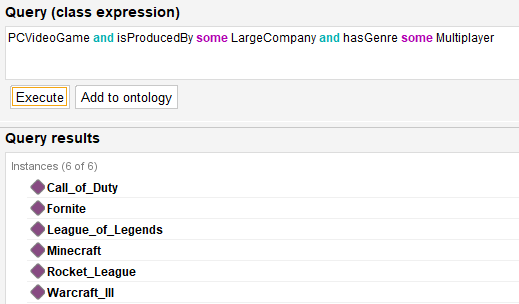
\includegraphics[scale=0.6]{query1}
  \caption{query of multiplayer video games made by large companies}
\end{figure}
\begin{figure}[h]
  \centering
  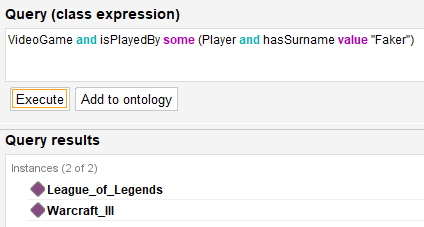
\includegraphics[scale=0.5]{query2}
   \caption{query of video games played by professional player "Faker"}
\end{figure}
\begin{figure}[h!]  
\centering
  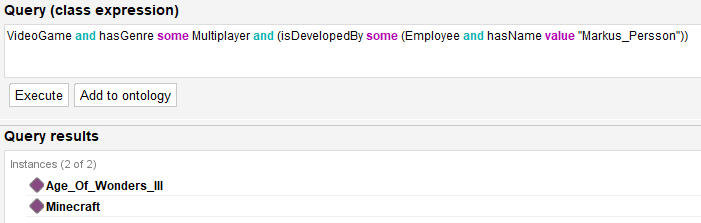
\includegraphics[scale=0.5]{query3}
   \caption{query of multiplayer video games made by famous developer "Markus Persson"}
\end{figure}

\subsection*{G.2 Evaluation}

The video games ontology has to provide the means for querying the games through the most relevant features at the time and given level of granularity it conveys we expect it to meet its initial goal. 

\subsection*{G.3 Value of use}

See queries in section testing G.1 Testing.
\subsection*{G.4 Institutional endorsement}
No particular institutional endorsement. 
\subsection*{G.5 Evidence of use}
Same type of ontology may be used by digital video games retail contenders such as Steam or Amazon. 
\\
\\
\\
\\
\\
\\


\section*{Appendix}

\begin{figure}[h]  
\centering
  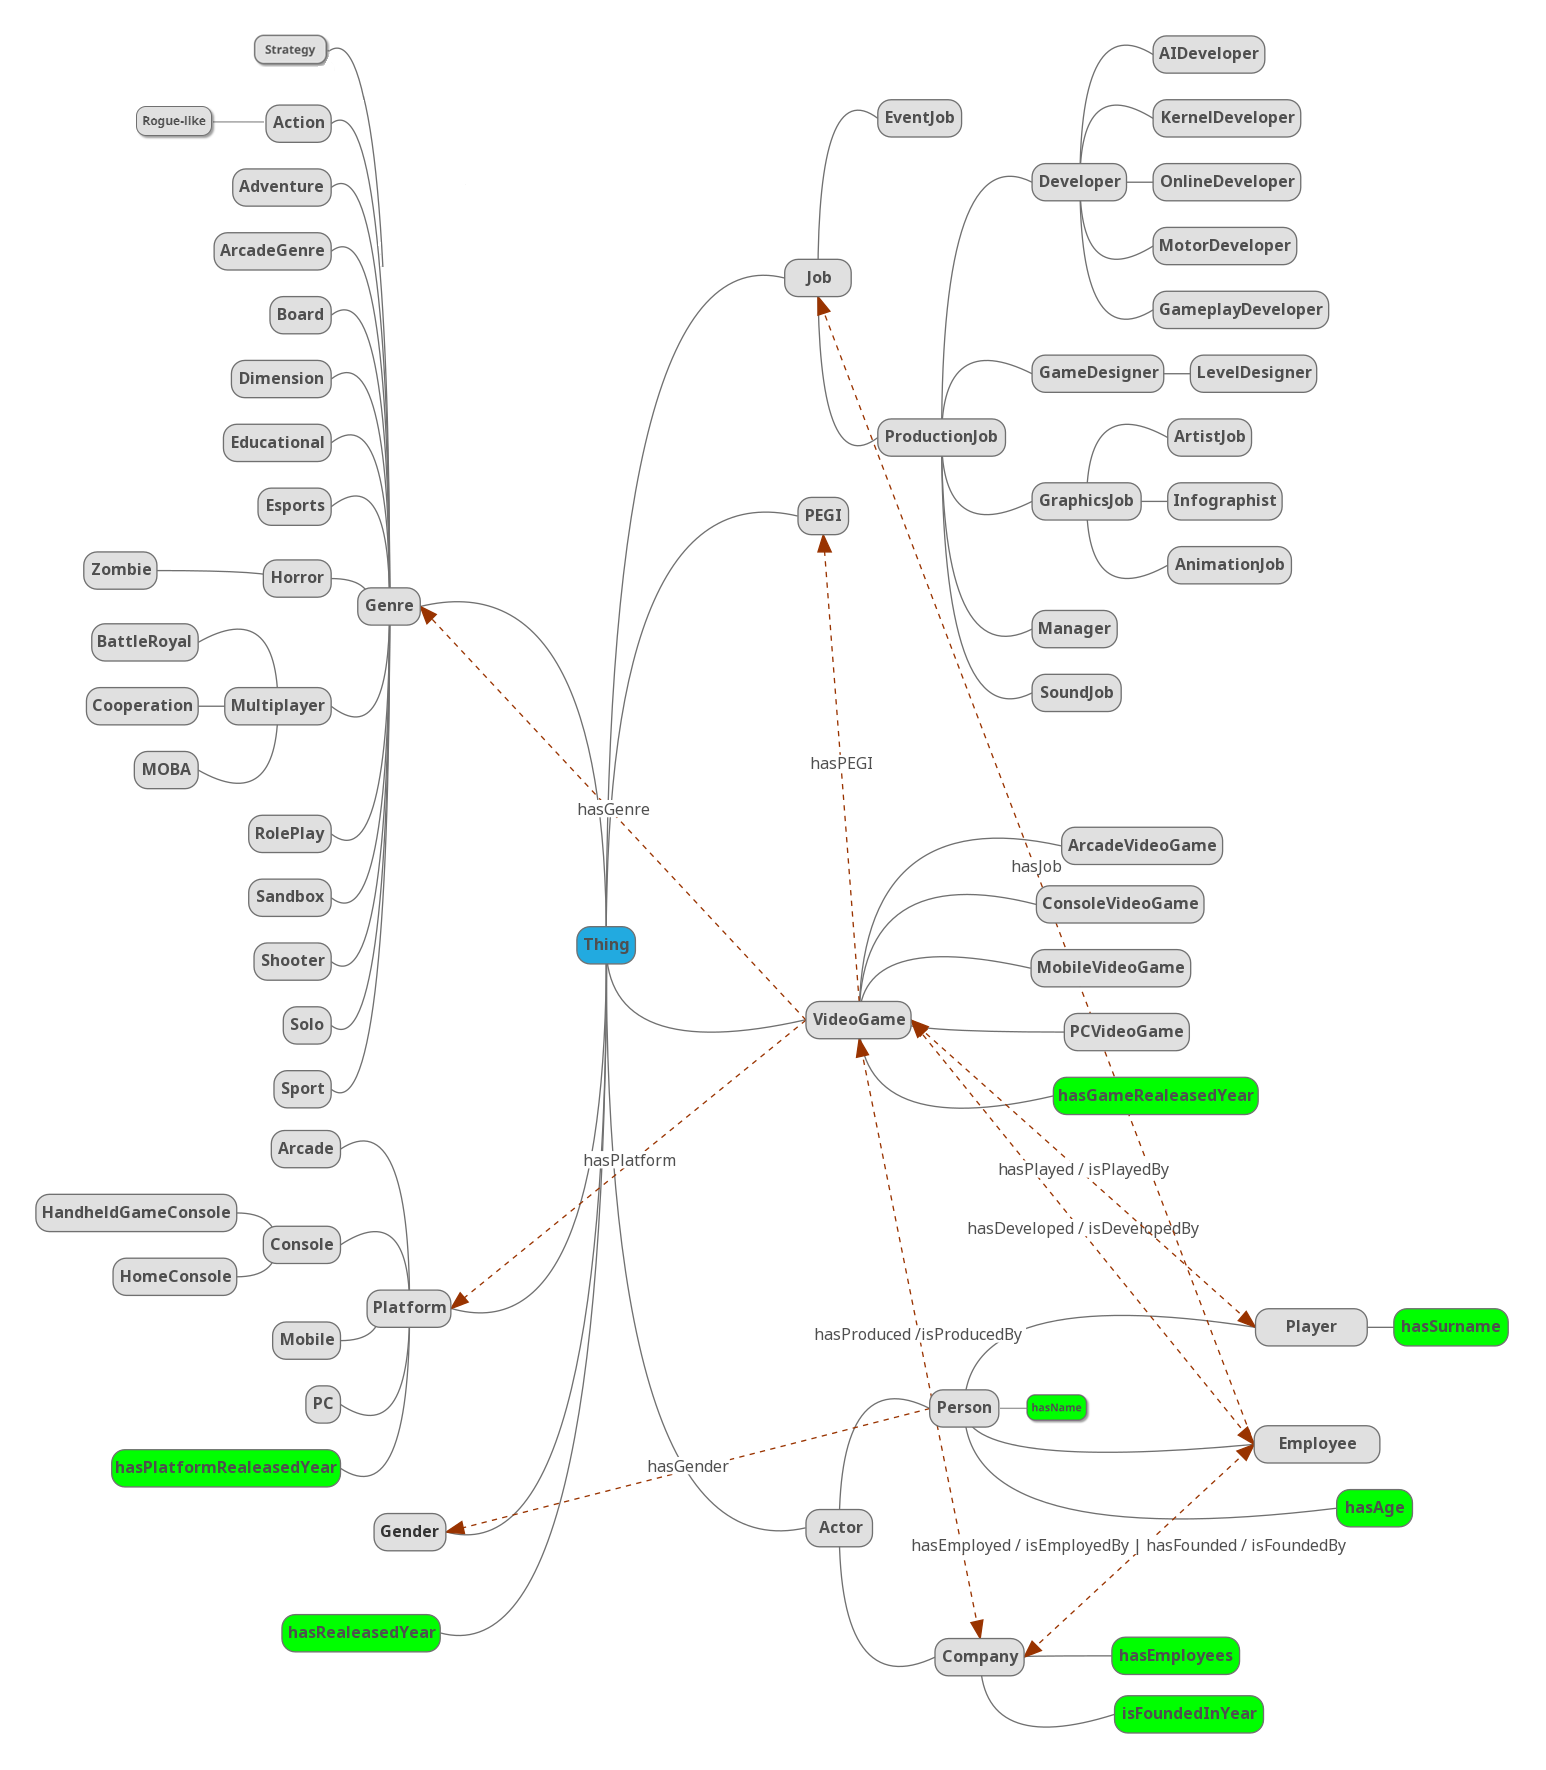
\includegraphics[scale=0.45]{ontologieV2}
   \caption{Ontology map}
\end{figure}


\end{document}
